\documentclass[xcolor={dvipsnames,table}]{beamer}
\usepackage{epsfig,graphicx}
\usepackage{palatino}
\usepackage{fancybox}
\usepackage{relsize}
\usepackage[procnames]{listings}
\usepackage{hyperref}
\usepackage{qtree} % needed?
\usepackage{booktabs}
\usepackage{dirtree}
\usepackage[normalem]{ulem}


% fatter TT font
\renewcommand*\ttdefault{txtt}
% another TT, suggested by Alex
% \usepackage{inconsolata}
% \usepackage[T1]{fontenc} % needed as well?


\newcommand{\scale}{0.7}

\newcommand{\todo}[1]{{\emph{TODO: #1}}}
\newcommand{\martin}[1]{{\color{blue} Martin: #1}}
\newcommand{\abcdef}[1]{{\color{red} Author2: #1}}

% uncomment following for final submission
%\renewcommand{\todo}[1]{}
%\renewcommand{\martin}[1]{}
%\renewcommand{\author2}[1]{}

\newcommand{\code}[1]{{\texttt{#1}}}

\hypersetup{
  linkcolor  = black,
%  citecolor  = blue,
  urlcolor   = blue,
  colorlinks = true,
}

\beamertemplatenavigationsymbolsempty
\setbeamertemplate{footline}[frame number]





\newif\ifbook
\input{../shared/chisel}

\title{Finite-State Machines}
\author{Martin Schoeberl}
\date{\today}
\institute{Technical University of Denmark\\
Embedded Systems Engineering}

\begin{document}

\begin{frame}
\titlepage
\end{frame}


\begin{frame}[fragile]{Overview}
\begin{itemize}
\item A bit of testing (repetition)
\item Fun with counters
\item Finite-state machines
\item Collection with \code{Vec}
\end{itemize}
\end{frame}

\begin{frame}[fragile]{Organization and Lab Work}
\begin{itemize}
\item How did the testing lab work? Did you find both bugs?
\item This week is the 7-segment decoder
\item This is part of the lab grade -- show it a TA
\begin{itemize}
\item Deadline is next week (100 \%)
\item In two weeks (21/3) only 50 \%
\end{itemize}
\item Register your group to get a number!
\begin{itemize}
\item Group name: VM Machine
\end{itemize}
\end{itemize}
\end{frame}

\begin{frame}[fragile]{Testing with Chisel}
\begin{itemize}
\item A test contains
\begin{itemize}
\item a device under test (DUT) and
\item the testing logic
\end{itemize}
\item Set input values with \code{poke}
\item Advance the simulation with \code{step}
\item Read the output values with \code{peek}
\item Compare the values with \code{expect}
\item Import following packages
\shortlist{../code/test_import.txt}
\end{itemize}
\end{frame}

\begin{frame}[fragile]{An Example DUT}
\begin{itemize}
\item A device-under test (DUT)
\item Just 2-bit AND logic
\shortlist{../code/test_dut.txt}
\end{itemize}
\end{frame}

\begin{frame}[fragile]{A ChiselTest}
\begin{itemize}
\item Extends class \code{AnyFlatSpec} with \code{ChiselScalatestTester}
\item Has the device-under test (DUT) as parameter of the \code{test()} function
\item Test function contains the test code
\item Testing code can use all features of Scala
\item Is placed in \code{src/test/scala}
\item Is run with \code{sbt test}
\end{itemize}
\end{frame}


\begin{frame}[fragile]{Testing with \code{expect()}}
\begin{itemize}
\item Poke values and \code{expect} some output
\shortlist{../code/test_bench.txt}
\end{itemize}
\end{frame}

\begin{frame}[fragile]{Call the Tester for Waveform Generation}
\begin{itemize}
\item The complete test
\item Note the \code{.withAnnotations(Seq(WriteVcdAnnotation)}
\end{itemize}
\begin{chisel}
class Count6WaveSpec extends AnyFlatSpec with ChiselScalatestTester {
  "CountWave6 " should "pass" in {
    test(new Count6).withAnnotations(Seq(WriteVcdAnnotation)) { dut =>
      dut.clock.step(20)
    }
  }
}
\end{chisel}
\end{frame}

\begin{frame}[fragile]{Display Waveform with GTKWave}
\begin{itemize}
\item Run the tester: \code{sbt test}
\item Locate the .vcd file in test\_run\_dir/...
\item Start GTKWave
\item Open the .vcd file with
\begin{itemize}
\item File -- Open New Tab
\end{itemize}
\item Select the circuit
\item Drag and drop the interesting signals
\end{itemize}
\end{frame}





\begin{frame}[fragile]{Counters as Building Blocks}
\begin{itemize}
\item Counters are versatile tools
\item Count events
\item Generate timing ticks
\item Generate a one-shot timer
\end{itemize}
\end{frame}

\begin{frame}[fragile]{Counting Up and Down}
\begin{itemize}
\item Up:
\shortlist{../code/when_counter.txt}
\item Down:
\shortlist{../code/down_counter.txt}
\end{itemize}
\end{frame}

\begin{frame}[fragile]{Generating Timing with Counters}
\begin{itemize}
\item Generate a \code{tick} at a lower frequency
\item We used it in Lab 1 for the blinking LED
\item Use it today for the lab exercise
\item Use it for driving the display multiplexing at 1~kHz
\end{itemize}
\begin{figure}
  \includegraphics[scale=0.8]{../figures/tick_wave}
\end{figure}
\end{frame}


\begin{frame}[fragile]{The Tick Generation}
\shortlist{../code/sequ_tick_gen.txt}
\end{frame}

\begin{frame}[fragile]{Using the Tick}
\begin{itemize}
\item A counter running at a \emph{slower frequency}
\item By using the \code{tick} as an enable signal
\end{itemize}
\shortlist{../code/sequ_tick_counter.txt}
\end{frame}

\begin{frame}[fragile]{The \emph{Slow} Counter}
\begin{itemize}
\item Incremented every \code{tick}
\end{itemize}
\begin{figure}
  \includegraphics[scale=0.8]{../figures/tick_count_wave}
\end{figure}
\end{frame}

\begin{frame}[fragile]{A Timer}
\begin{itemize}
\item Like a kitchen timer
\item Start by loading a timeout value
\item Count down till 0
\item Assert \code{done} when finished
\end{itemize}
\end{frame}

\begin{frame}[fragile]{One-Shot Timer}
\begin{figure}
  \includegraphics[scale=\scale]{../figures/timer}
\end{figure}
\end{frame}

\begin{frame}[fragile]{One-Shot Timer}
\shortlist{../code/timer.txt}
\end{frame}

\begin{frame}[fragile]{A 4 Stage Shift Register}
\begin{figure}
  \includegraphics[scale=\scale]{../figures/shiftregister}
\end{figure}
\shortlist{../code/shift_register.txt}
\end{frame}


\begin{frame}[fragile]{A Shift Register with Parallel Output}
\begin{figure}
  \includegraphics[scale=\scale]{../figures/shiftreg-paraout}
\end{figure}
\shortlist{../code/shift_paraout.txt}
\end{frame}

\begin{frame}[fragile]{A Shift Register with Parallel Load}
\begin{figure}
  \includegraphics[scale=0.5]{../figures/shiftreg-paraload}
\end{figure}
\shortlist{../code/shift_paraload.txt}
\end{frame}



\begin{frame}[fragile]{A Simple Circuit}
\begin{itemize}
\item What does the following circuit?
\item Is this related to a finite-state machine?
\end{itemize}
\begin{figure}
  \includegraphics[scale=\scale]{../figures/fsm-rising}
\end{figure}
\end{frame}

\begin{frame}[fragile]{Before the Break}
\begin{itemize}
\item Let us talk about AI tools
\end{itemize}
\end{frame}

\begin{frame}[fragile]{ChatGPT/Copilot}
\begin{itemize}
\item Maybe useful to learn a language
\item Sometimes ChatGPT uses old Chisel constructs
\item Sometimes it is even plain wrong
\item DTU does not allow the usage at the exam
\begin{itemize}
\item We will have the exam online without Internet access
\end{itemize}
\item My personal opinion:
\begin{itemize}
\item It is just a new tool
\item We cannot really (and shall not) disallow tools (grammar check, calculator, programming,...)
\item We will need to learn how to deal with it
\item I use Copilot in my editor
\item Sometimes I use ChatGPT to rewrite text
\end{itemize}
\end{itemize}
\end{frame}

\begin{frame}[fragile]{ChatGPT/Copilot}
\begin{itemize}
\item This morning I tried to solve todays lab with ChatGPT (3.5)
\item It took me 4 prompts and one correction prompt
\item The result looks correct
\item Done in 10 minutes
\item Can one learn to code with ChatGPT? Even better?
\item I do not know
\end{itemize}
\end{frame}

\begin{frame}[fragile]{Finite-State Machine (FSM)}
\begin{itemize}
\item Has a register that contains the state
\item Has a function to computer the next state
\begin{itemize}
\item Depending on current state and input
\end{itemize}
\item Has an output depending on the state
\begin{itemize}
\item And maybe on the input as well
\end{itemize}
\item Every synchronous circuit can be considered a finite state machine
\item However, sometimes the state space is a little bit too large
\end{itemize}
\end{frame}

\begin{frame}[fragile]{Basic Finite-State Machine}
\begin{itemize}
\item A state register
\item Two combinational blocks
\end{itemize}
\begin{figure}
  \includegraphics[scale=\scale]{../figures/fsm}
\end{figure}
\end{frame}

\begin{frame}[fragile]{State Diagram}
\begin{figure}
  \includegraphics[scale=\scale]{../figures/state-diag-moore}
\end{figure}
\begin{itemize}
\item States and transitions depending on input values
\item Example is a simple alarm FSM
\item Nice visualization
\item Will not work for large FSMs
\item Complete code in the Chisel book
\end{itemize}
\end{frame}


\begin{frame}[fragile]{State Table for the Alarm FSM}
\begin{table}
\centering
\begin{tabular}{ccccc}
\toprule
& \multicolumn{2}{c}{Input} \\
\cmidrule{2-3}
State &  Bad event & Clear & Next state & Ring bell \\
\midrule
green & 0 & 0 & green & 0 \\
green & 1 & - & orange & 0 \\
orange & 0 & 0 & orange & 0 \\
orange & 1 & - & red & 0 \\
orange & 0 & 1 & green & 0 \\
red & 0 & 0 & red & 1 \\
red & 0 & 1 & green & 1 \\
\bottomrule
\end{tabular}
\label{tab:state:table}
\end{table}
\end{frame}

\begin{frame}[fragile]{The Input and Output of the Alarm FSM}
\begin{itemize}
\item Two inputs and one output
\end{itemize}
\shortlist{../code/simple_fsm_io.txt}
\end{frame}

\begin{frame}[fragile]{Encoding the State}
\begin{itemize}
\item We can optimize state encoding
\item Two common encodings are: binary and one-hot
\item We leave it to the synthesize tool
\item Use symbolic names with \code{ChiselEnum}
\end{itemize}
\shortlist{../code/simple_fsm_states.txt}
\end{frame}

\begin{frame}[fragile]{Start the FSM}
\begin{itemize}
\item We have a starting state on reset
\end{itemize}
\shortlist{../code/simple_fsm_register.txt}
\end{frame}


\begin{frame}[fragile]{The Next State Logic}
\shortlist{../code/simple_fsm_next.txt}
\end{frame}

\begin{frame}[fragile]{The Output Logic}
\shortlist{../code/simple_fsm_output.txt}
\end{frame}

\begin{frame}[fragile]{Summary of the Alarm Example}
\begin{itemize}
\item Three elements:
\begin{enumerate}
\item State register
\item Next state logic
\item Output logic
\end{enumerate}
\item This was a so-called Moore FSM
\item There is also a FSM type called Mealy machine
\end{itemize}
\end{frame}

\begin{frame}[fragile]{A so-called Mealy FSM}
\begin{itemize}
\item Similar to the former FSM
\item Output also depends in the input
\item It can react \emph{faster}
\item Less composable (draw it)
\end{itemize}
\begin{figure}
  \includegraphics[scale=\scale]{../figures/mealy}
\end{figure}
\end{frame}

\begin{frame}[fragile]{The Mealy FSM for the Rising Edge}
\begin{itemize}
\item That was our starting example
\item Output is also part of the transition arrows
\end{itemize}
\begin{figure}
  \includegraphics[scale=\scale]{../figures/state-diag-mealy}
\end{figure}
\end{frame}

\begin{frame}[fragile]{The Mealy Solution}
\begin{itemize}
\item Show code in IntelliJ as it is too long for slides
\end{itemize}
\end{frame}

\begin{frame}[fragile]{State Diagram for the Moore Rising Edge Detection}
\begin{itemize}
\item We need three states
\end{itemize}
\begin{figure}
  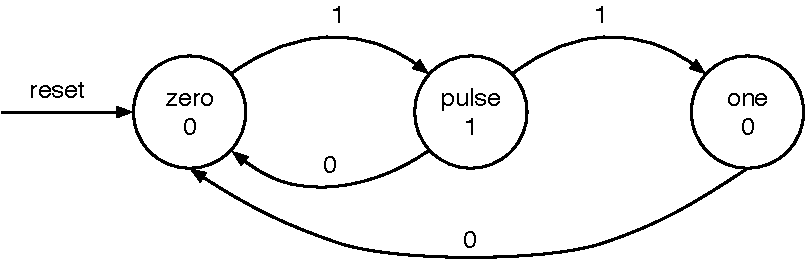
\includegraphics[scale=\scale]{../figures/state-diag-rising-moore}
\end{figure}
\end{frame}

\begin{frame}[fragile]{Comparing with a Timing Diagram}
\begin{itemize}
\item Moore is delayed one clock cycle compared to Mealy
\end{itemize}
\begin{figure}
  \includegraphics[scale=1]{../figures/rising}
\end{figure}
\end{frame}

\begin{frame}[fragile]{What is Better?}
\begin{itemize}
\item It depends ;-)
\item Moore is on the save side
\item More is composable
\item Mealy has \emph{faster} reaction
\item Both are tools in you toolbox
\item Keep it simple with your vending machine and use a Moore FSM
\end{itemize}
\end{frame}

\begin{frame}[fragile]{Another Simple FSM}
\begin{itemize}
\item a FSM for a single word buffer
\item Just two symbols for the state machine
\end{itemize}
\begin{chisel}
  object State extends ChiselEnum {
    val empty, full = Value
  }
\end{chisel}
\end{frame}

\begin{frame}[fragile]{Finite State Machine for a Buffer}
\begin{chisel}
  object State extends ChiselEnum {
    val empty, full = Value
  }
  import State._

  val stateReg = RegInit(empty)
  val dataReg = RegInit(0.U(8.W))

  when(stateReg === empty) {
    when(io.in.valid) {
      dataReg := io.in.bits
      stateReg := full
    }
  } .otherwise { // full
    when(io.out.ready) {
      stateReg := empty
    }
  }
\end{chisel}
\begin{itemize}
\item A simple buffer for a bubble FIFO
\end{itemize}
\end{frame}


\begin{frame}[fragile]{Group Signals with a \code{Bundle}}
\begin{itemize}
\item Group signals that belong to each other
\item Reference as a whole
\item Individual fields accessed by their name
\item E.g., \code{ref.field}
\end{itemize}
\shortlist{../code/bundle.txt}
\end{frame}

\begin{frame}[fragile]{A Collection of Signals with \code{Vec}}
\begin{itemize}
\item Chisel \code{Vec} is a collection of signals of the same type
\item The collection can be accessed by an index
\item Similar to an array in other languages
\item Wrap into a \code{Wire()} for combinational logic
\item Wrap into a \code{Reg()} for a collection of registers
\end{itemize}
\shortlist{../code/vec.txt}
\end{frame}

\begin{frame}[fragile]{Using a \code{Vec}}
\shortlist{../code/vec_access.txt}
\begin{itemize}
\item Reading from an \code{Vec} is a multplexer
\item We can put a \code{Vec} into a \code{Reg}
\end{itemize}
\shortlist{../code/reg_file.txt}
\noindent An element of that register file is accessed with an index and used as a normal register.

\shortlist{../code/reg_file_access.txt}
\end{frame}


\begin{frame}[fragile]{Mixing Vecs and Bundles}
\begin{itemize}
\item We can freely mix bundles and vectors
\item When creating a vector with a bundle
type, we need to pass a prototype for the vector fields. Using our
\code{Channel}, which we defined above, we can create a vector of channels with:
\end{itemize}
\shortlist{../code/vec_bundle.txt}
\begin{itemize}
\item A bundle may as well contain a vector
\end{itemize}
\shortlist{../code/bundle_vec.txt}
\end{frame}

\begin{frame}[fragile]{Today's Lab}
\begin{itemize}
\item This is the start of the graded group work
\begin{itemize}
\item Part of your grade
\item Please register your group in DTU Learn
\end{itemize}
\item Binary to 7-segment decoder
\item First part of your vending machine
\item Just a single digit, only combinational logic
\item Use the nice tester provided to develop the circuit
\item Then synthesize it for the FPGA
\item Test with switches
\item Then add a counter running at 2 Hz
\item Show a TA your working design
\item \href{https://github.com/schoeberl/chisel-lab/tree/master/lab5}{Lab 5}
\end{itemize}
\end{frame}



\begin{frame}[fragile]{Summary}
\begin{itemize}
\item Waveform testing is the way to develop/debug
\item Counters are important tools, e.g., to generate timing
\item Finite-state machines are another tool of the trade
\item Two types: Moore and Mealy
\item A Chisel \code{Vec} is the hardware version of an array
\end{itemize}
\end{frame}


\end{document}

%\begin{frame}[fragile]{xxx}
%\begin{itemize}
%\item yyy
%\end{itemize}
%\end{frame}
